The performance analysis will be accomplished in multiple segments. To begin with the assessment, we do the analysis in each frame work using different algorithms and different cluster settings. Following that a performance assessment between the frameworks will be conducted to obtain a  proper idea on how these two frameworks can perform in pretty similar situations. To calculate the performance of the algorithms we used \emph{linux verbose} command.

\subsection{performance analysis on Hadoop}
To execute the performance analysis multiple versions of the code has been prepared and run using Hadoop cluster individually on different cluster settings which is discussed on \ref{sec:background}. Linux command \emph{command time --verbose} has been used at the start of Hadoop command to register the time and resource usage. The results for different methods and settings can be found in Figure~\ref{fig:hPerformance}. By taking a look through the numbers of the performance analysis table, it's understood that regEx and statistic function do a much better job in terms of using system resources because the results show that the settings which has been used them has been implemented in a shorter time in comparison to other two methods. And also as you can see the setting with 5 worker node in the cluster has much better performance rather than the cluster setting with 3 worker nodes.

\subsection{Performance analysis Spark}
The same as Hadoop multiple versions of codes has been implemented on Spark using different cluster settings and the time of implementation has been registered you can find the table for Spark performance assessment in Figure~\ref{fig:sPerformance}. As can be seen in the table, performance of the algorithm which use textblob as the implementation tool for sentiment analysis is extensively higher than non-trivial algorithm used in other methods. Also as we expected the implementation time drastically decreases when two more worker node is added to the cluster.
Also using regEx and python built-in functions alternatively affects on the running time which shows regEx is slightly more efficient. 



\subsection{Hadoop vs Spark Performance assessment}
Although at least in our case except the sentiment analysis part which seems more difficult in Hadoop as we faced issues importing libraries in Hadoop in the proper way, implementing simple MRJob functions seems much easier in Hadoop because of the better performance of the reducer (maybe our experience was because of the fact that we didn't spend as much time on Spark as we spent on learning Hadoop), the performance in Spark is insanely higher and also Spark is more widely used by the companies in enterprise projects and also as the cloud frameworks like Databricks is built upon Spark and has been using around the world it seems Spark will be the winner of the future. But in terms of the performance, as you can see in Figure the performance of Hadoop is considerably higher in the same cluster setting, algorithm and data-set. we specifically tried to have the same code on two framework to have a legit comparison. In Figure~\ref{fig:hvss}we tried to compare two frameworks with the same settings and code and as you can see Spark performs likely 3 times better than Hadoop.
\begin{figure}[t]
   \centering
   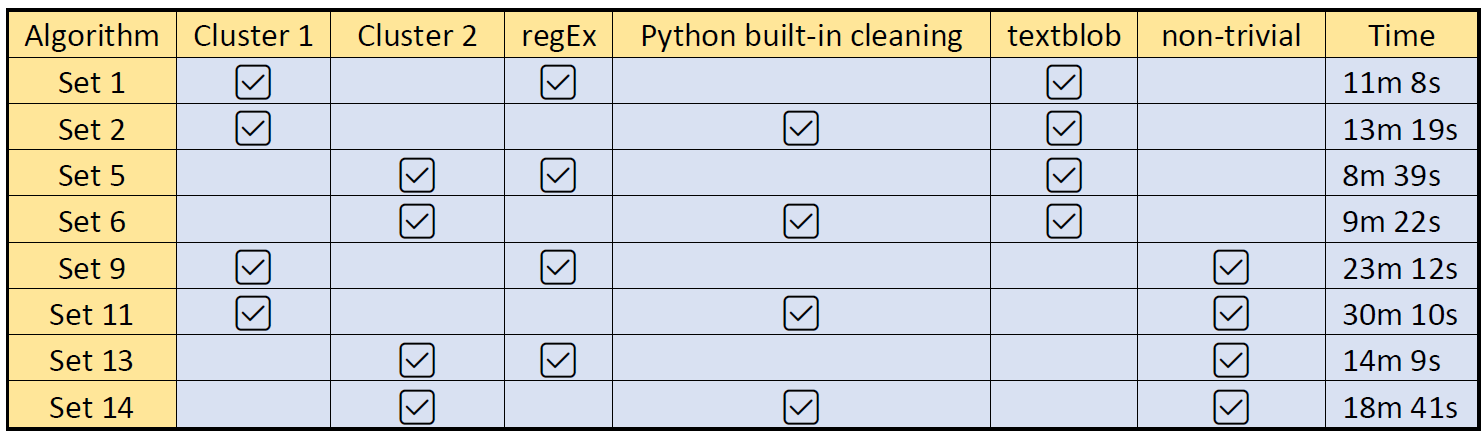
\includegraphics[width=\linewidth]{fig/sPerformance.png}
    \caption{Spark Performance statistics}
    \label{fig:sPerformance}
\end{figure}


\begin{figure}[t]
   \centering
   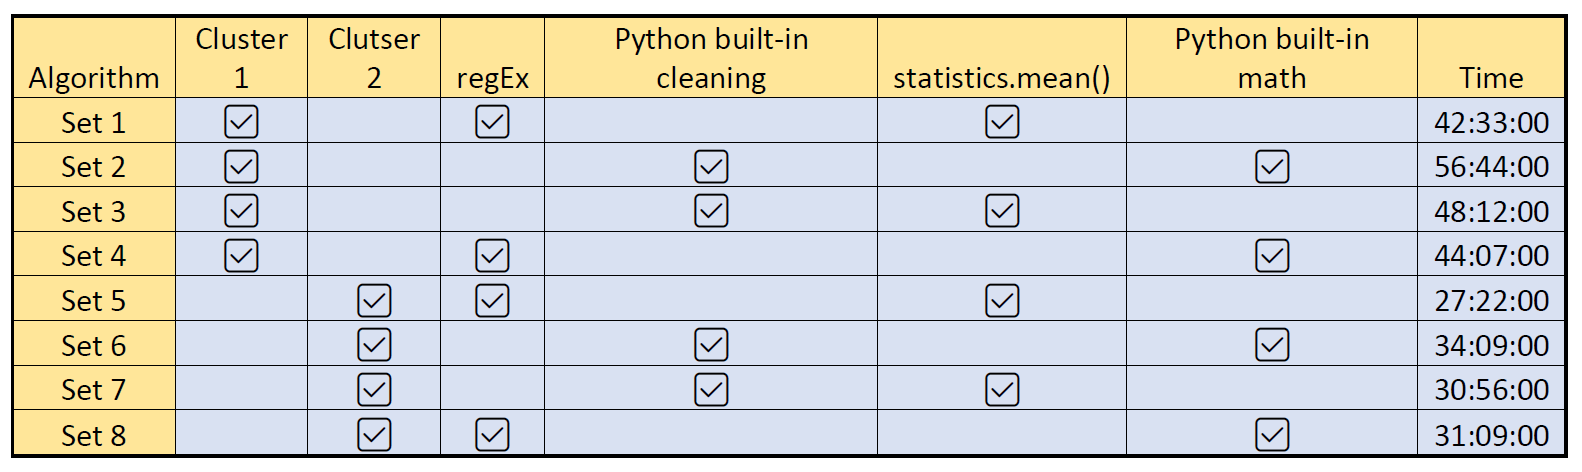
\includegraphics[width=\linewidth]{fig/hPerformance.png}
    \caption{Hadoop Performance statistics}
    \label{fig:hPerformance}
\end{figure}


\begin{figure}[t]
   \centering
   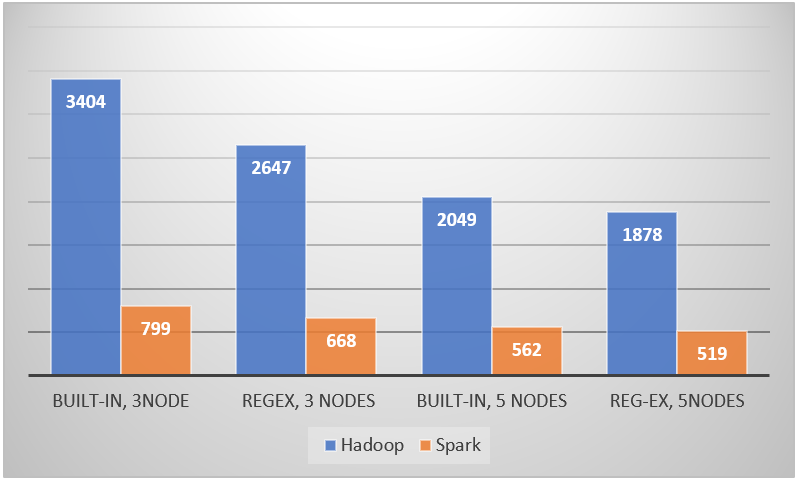
\includegraphics[width=\linewidth]{fig/hvss.png}
    \caption{Hadoop vs Spark}
    \label{fig:hvss}
\end{figure}